\documentclass[a0,portrait]{a0poster}

% Switch off page numbers on a poster, obviously, and section numbers too.
\pagestyle{empty}
\setcounter{secnumdepth}{0}

% The textpos package is necessary to position textblocks at arbitary 
% places on the page.
\usepackage[absolute]{textpos}

\usepackage{graphics,wrapfig}
\usepackage{palatino}
\usepackage{color}

\let\Textsize\normalsize
%\def\Subhead#1{\noindent{\large #1}}

\def\Title#1{\noindent{\Huge #1}}
\def\Head#1{\noindent{\LARGE #1}\bigskip \\}
\def\Authors#1{\noindent{\large #1}\smallskip}

% Set up the grid
%
% Note that [40mm,40mm] is the margin round the edge of the page --
% it is _not_ the grid size. That is always defined as 
% PAGE_WIDTH/HGRID and PAGE_HEIGHT/VGRID. In this case we use
% 15 x 25. This gives us a wide central column for text (7 grid
% spacings) and two narrow columns (3 each) at each side for 
% pictures, separated by 1 grid spacing.
%
% Note however that texblocks can be positioned fractionally as well,
% so really any convenient grid size can be used.
%
\TPGrid[80mm,80mm]{15}{25}  % 3 - 1 - 7 - 1 - 3 Columns

\parindent=0pt
\parskip=0.5\baselineskip

\begin{document}
\fontsize{40pt}{60pt}\selectfont

\begin{textblock}{12}(0,0)
\baselineskip=3\baselineskip \Title{Fitting an All-atom Protein Model to a $C_\alpha$-trace}
\end{textblock}

\begin{textblock}{12}(0, 0.6)
\Authors{Martin Dybdal, Anders Boesen Lindbo Larsen and Esben Skaarup}
\end{textblock}

% Put the KU logo in the top right.
% \begin{textblock}{2}(13,0)
% \includegraphics{ku-logo.pdf}
% \end{textblock}

\begin{textblock}{7}(0,2)

    \Head{Motivation}
Proteins are the perhaps most important molecules of living
organisms. They perform a multitude of biological tasks and are found
in all lifeforms, from bacteria and unicellular organisms to
multicellular organisms such as animals. The chemical abilities and
biological functions of proteins are determined by their
three-dimensional structure. The ability to determine this structure
without performing costly experiments will have many applications in
medicine (e.g. drug design) and biotechnology. Protein structure
prediction and the related topic protein folding\footnote{The two
  research fields are distinguished by whether the actual folding
  process is simulated (protein folding) or a legal structure is
  sought without computing the intermediate steps (protein structure
  prediction).} are large and active research fields. It is still an
open problem.

\end{textblock}

\begin{textblock}{7}(8,14)
  \Head{Introduction}
  

\end{textblock}



% If you want to add a figure do something like this:

\begin{textblock}{3}(0,15)
 \begin{center}
\resizebox{10\TPHorizModule}{!}{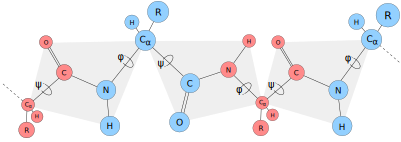
\includegraphics{../rapport/figures/protein-torsion-angles.pdf}}
\\\textbf{Figure 1}: Protein torsion angles
 \end{center}
\end{textblock}


\end{document}

